\documentclass[12pt,a4paper]{report}
\linespread{1.5}
\usepackage[hidelinks,colorlinks=false]{hyperref}
\usepackage[titletoc,title]{appendix}
\usepackage[nottoc]{tocbibind}
\usepackage{graphicx}
\usepackage{makeidx}
\usepackage{setspace}
\usepackage[margin=1.0in]{geometry}
\usepackage{authblk}
\usepackage{rotating}
\usepackage{cleveref}
\usepackage{float}
\usepackage{amsmath}
\usepackage{listings}
\usepackage{tikz}
\usetikzlibrary{arrows}
\graphicspath{{images/}}

\floatstyle{ruled}
\newfloat{program}{thp}{lop}
\floatname{program}{Program}
 
\begin{document}
	
	\title{Final Year Project Report\\ Development and implementation dynamic balance algorithms for bipedal robot locomotion.}
	\author{Usvyatsov Mikhail\\Innopolis University\\Kazan\\  ~\\ \normalsize Supervisor: Prof. Evgeni Magid}
	\date{\normalsize \today}
	\maketitle
	
	\tableofcontents
	
	\newpage

	\chapter{Introduction and Overview}
		Nowadays humanity has invented almost all devices that are needed for modern humans and society in general. Science is now engaged in the improvement and optimization of existing solutions. These solutions can be traced with trends that are repeated and replicated. This approach is quite good: gain experience, accumulate knowledge and apply them to the latest developments.
		
		According to \cite{pfeifer2007self} it is very important to consider the level of uncertainty of the environment where a robot works, because its body will interact with this environment. It was a common belief before the advent of industrial robots that robots should look like humans. The first use of the word "robot" refers to a humanoid machine that was supposed to serve a human. However, from the very beginning almost every automatic device intended for production and other operations normally performed by the human was called robot. Intensive development of robots started after the Second World War, which was associated with the emergence of the nuclear industry.
		
		The word robot was initially attributed in 1921 to fictional humanoid by Karel Capaek. Nowadays almost every professor teaching robotics can give their own definition of robots and all of them will not be similar. One of robot today's definition is autonomous device that work in automatic mode. It can be attributed to the machine "Lunokhod-1", created in 1966. It was the first machine in the history that worked on the surface of the Moon (1970). Another modern definition is a mechanical or virtual artificial agent, usually an electro-mechanical machine that is guided by a computer program or electronic circuitry.
		
		Lately robots began to replace humans not only in manufacturing but also in the military sphere. Constantly emerging information about the achievements of the leading countries in the development of military land, underwater robots and unmanned aerial vehicles is evidenced for this thesis. Bipedal humanoid walking robots comprise the area of robotics that is developing most rapidly nowadays.
		
		The trend towards automation is a core part of progress. Automation reduces the cost of technical processes and the risk to humans. Therefore, the research and development for this task are on the cutting edge of science and technology and require special attention and investment into its development. There are more and more situations requiring people to perform a wide variety of work in heavy, dangerous, and sometimes incompatible with the life conditions. In response, there are new tools of extreme robotics. However, for the most part they are very similar to each other. Usually, autonomous wheeled or tracked vehicles with manipulators are used to perform tasks on the ground. Mostly these robots are teleoperated. These robots are being produced for more than a dozen years. Engineers have so far accumulated a lot of experience in their development and applications, which are in some cases very efficient. However, it is obvious that this technique has (like any other) a limited scope of application. People still have to work in dangerous conditions such as in chemical, biological, or radioactive hazards, work in extremely hot or cold conditions, fight against criminals and terrorist.
		Human workspace is very specific due to people's two arms and two legs. Universal robot should operate in the same environment and workspace. For this reason other areas of extreme robotics are developing now.
		One of these is a robotic system including an anthropomorphic bipedal walking robot. Such robot's kinematics, size and weight are similar to human's, it is equipped with an energy source, communication channel with the control station, and a powerful autonomous control system, allowing it to perform actions in supervisory or automatic mode. For instance, autonomous actions include independent movement from place to place in absence of communication. Such robots have significant advantages in workspaces initially adapted for humans.

	\chapter{Literature review}
		Bipedal locomotion is a very complex task and according to \cite{erbatur2002study} it is described by nontrivial dynamics. It still doesn't have complete general solution however the research of this has a long history. The development of the models starts from the inverted pendulum model of human walking and goes to the complex approach of actuated passive walking with ZMP control.\\
		According to \cite{wright2014intelligent}, there are 5 groups of approaches to the problem of locomotion control. There are:
		
		\begin{enumerate}
			\item Analytical.\\ It uses equations of physical values to generate walking trajectories.
			\item Central Pattern Generator (CPG).\\ When biologically inspired creature walks it has two different mechanisms of motion control. CPG is analog of generator that produces the pattern that doesn't require to be adopted. And also control mechanism applied to generated by CPG pattern with external data from sensors as input make the movement to be adopted to very big variety of disturbances.
			\item Neural Networks.\\ This approach is a try of simulating the control process of biologically inspired creatures.
			\item Hidden Markov Model (HMM).\\ HMM are good for pattern recognition, thus we can use it to recognize patterns in gaits.
			\item Rule based.\\ The main idea behind this approach is to build the rules for all possible variations of configuration.
		\end{enumerate}

		\section{Analytical approach}
		The oldest one and also the most studied group is analytical one. It requires the knowledge of general form that locomotion should take.

		For bipedal locomotion it s required to accomplish the following steps \cite{wright2014intelligent}:
		\begin{enumerate}
			\item Apply stability constraints
			\item Design gait algorithm (including double support, single support and no-support phases).
			\item Solve remaining degrees of freedom (DoF) with Inverse Kinematics (IK).
		\end{enumerate}

		According to \cite{tang2008analysis}, the most natural method that represents the human body is inverted pendulum.
		Inverted pendulum model of human balance problem is one of the most primitive and old example of analytical approach \cite{winter1995human}. It stated that control of the balance can be achieved with two components: ankle mechanism (invertors/evertors) and hip load/unloading mechanism. In different positions each of the mechanism plays a different role. Thus in tandem or intermediate position balance is achieved by invertors/evertors mechanism while direction is controlled by hip load/unloading mechanism. It doubts on commonly used condition: reaction force of the floor has to go thought center of gravity of the robot. It was stated, that modern bio-mechanical studies show that there are angular moments around center of gravity. 
		Thus this approach is too approximate and it is not very accurate.
		Moreover, according to \cite{kuo2007six} six determinants theory\cite{inman1953major} well described by inverted pendulum model needs more energy to control the mechanism and this problem can be solved by passive dynamic walking machines, that need external energy only for transition from one pendular stance leg to another. In \cite{collins2005bipedal} such architecture was considered. There robot was able to move forward at constant not very high speed and author mentioned that the gait of the robot was human like. Human-like gait is desirable because of its energy effectiveness \cite{golliday1977approach}.\\
		Furthermore, \cite{anderson2005powered} summaries principles that allows to combine passive dynamic control with powered bipeds. The results show that the gait become energy efficient however it implies further work on robustness and flexibility of walking\\

		In 1970 Miomir Vukobratovic proposed Zero Moment Point (ZMP), a theoretical model to explain biped locomotion. Also ZMP is a basic dynamical stability constraint.
		According to \cite{manchester2011stable} we can divide all the existing humanoid bipedal walking robots into two big groups: ZMP-controlled ones and passive - dynamic walkers.\\
		Zero moment point is a concept related with dynamics and control of legged locomotion for humanoid robots. It specifies the point with respect to which dynamic reaction force at the contact of the foot with the ground does not produce any moment in the horizontal direction, i.e. the point where the total of horizontal inertia and gravity forces equals to zero.
		Miomir Vukobratovic in \cite{vukobratovic2004zero} defines ZMP (Zero Moment Point) as a point in which we can reduce all the forces and moments with one single force $F_a$ and moment $M_a$ respectively  \cref{fig:1}.
	
		\begin{figure}[h!]
			\vspace{-0.2cm}
			\centering
			{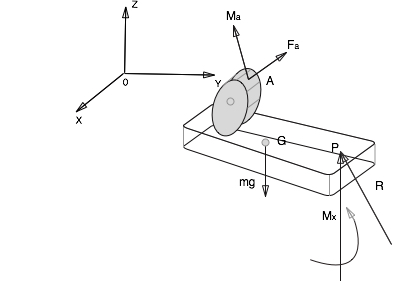
\includegraphics[width=0.7\textwidth]{1}}
			\caption{The sole with acting forces on it}
			\label{fig:1}
			\vspace{-0.1cm}
		\end{figure}

		On the figure above we consider only the sole separately from other parts of the leg. It has its own center of gravity G. At point P there is resulting ground reaction that maintains the construction in the equilibrium. The force of ground reaction R and moment M consists of its three components ($R_x$, $R_y$, $R_z$) and ($M_x$, $M_y$, $M_z$) respectively. Horizontal components of R should compensate friction force in the point of contact. Thus, the horizontal reaction of force ($R_x$, $R_y$) represents 
		friction force that compensate horizontal component of $F_a$. In the same time the moment $M_z$ represents friction reaction forces \cref{fig:2} that compensates vertical component of $M_a$ and the moment induced by $F_a$. \cite{vukobratovic2004zero}

		\begin{figure}[h!]
			\vspace{-0.2cm}
			\centering
			{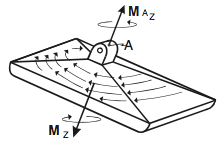
\includegraphics[width=0.7\textwidth]{2}}
			\caption{Rotational moment in the sole}
			\label{fig:2}
			\vspace{-0.1cm}
		\end{figure}

		According to \cite{kajita2003biped}, this ZMP should be on the foot. The problem is that we cannot manipulate the foot directly \cite{mitobe2000control}. According to \cite{vukobratovic2004zero} we can do it by ensuring the appropriate dynamics of the mechanism above the foot. If the resulting force in ZMP lies not in vertical direction (conditions from the paragraph above doesn't hold and R and $M_z$ doesn't compensate correspondent components of $F_a$ and $M_a$) than foot will slide. It means that dynamical stability was not achieved due to the fact, that there is a rotational moment that will affect the robot. On the other hand, in \cite{sardain2004forces} it was proven: if ZMP was achieved in the polygon of foot and moreover it coincides with the contact point, than robot is stable, due to the fact, that all the resulting forces lies in vertical direction. During the walk the position of ZMP should be computed simultaneously and the main problem of control is to keep ZMP and contact point to be coincided inside the support polygon of contact foot with the ground.
		The name zero moment point relates to the fact, that dynamical stability is maintained if horizontal components $M_x$ and $M_y$ are both equal to zero.
	
		\begin{equation}\label{eq:ZMP1}
			M_x = M_y = 0
		\end{equation}

		In the point P there should exist such equivalent force R and vertical moment $M_z$ that compensate the force reaction of the ground and maintains the stability of the construction. If we want to achieve the dynamical stability, that the following equations holds:

		\begin{equation}\label{eq:ZMP2}
			R + F_a + mg = 0
		\end{equation}

		Where $m$ is a foot mass. In \cite{vukobratovic2004zero} there is defined  point O - the origin coordinates frame from which we can define radius vectors $\vec{OP}$, $\vec{OG}$ and $\vec{OA}$ where A is a point of ankle joint.

		\begin{equation}\label{eq:ZMP3}
			\vec{OP} \times \vec{R} + \vec{OG} \times mg + M_A + M_z + \vec{OA} \times F_a = 0
		\end{equation}

		Placing the origin frame into the point P and making a projection on the horizontal plane gives us the following equations: 

		\begin{equation}\label{eq:ZMP4}
			(\vec{OP} \times \vec{R})^H + \vec{OG} \times mg + M_A^H + (\vec{OA} \times F_a)^H = 0
		\end{equation}

		According to \cite{vukobratovic2004zero} equation \ref{eq:ZMP4} represents the foot equilibrium. However ot doesn't solve the problem, that it is still unknown whether for the given motion of mechanism it is in the equilibrium. It is only of ZMP lies inside the support polygon.
		
		In \cite{dekker2009zero} it was stated, that we have to make the following assumptions in order to compute the position of ZMP:

		\begin{enumerate}
			\item
				The bipedal robot consists of n rigid links.
			\item
				All kinematic information, such as position of CoM, link orientation, velocities, etc. are known and calculated by forward kinematics.
			\item
				The floor is rigid and motionless.
			\item
				The feet cannot slide over the floor surface.
			\item
				All joints are actively actuated.
		\end{enumerate}
	
		With this constraints we can define the mass of the robot as:
	
		\begin{equation}\label{eq:ZMP5}
			m_{robot} = \sum^n_{i=1}{m_i}
		\end{equation}

		In \cite{dekker2009zero} it was considered schematic bipedal robot to derive the coordinates of ZMP [Fig. 3]

		\begin{figure}[h!]
			\vspace{-0.2cm}
			\centering
			{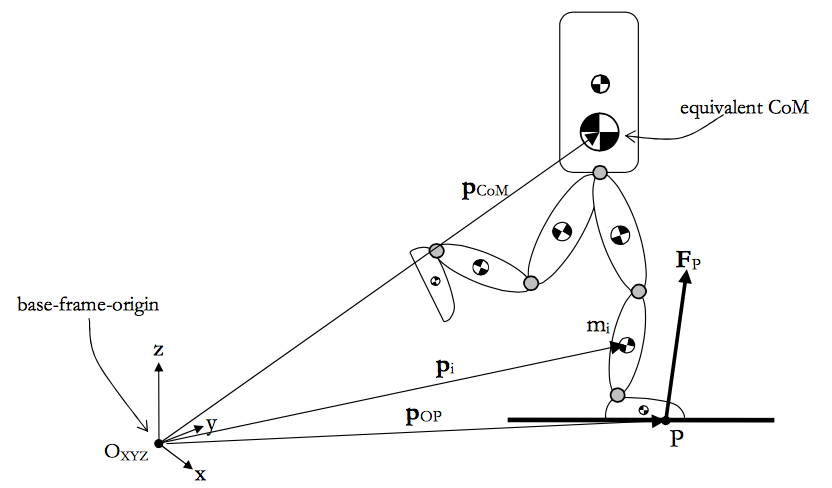
\includegraphics[width=0.7\textwidth]{3}}
			\caption{Rotational moment in the sole \cite{dekker2009zero}}
			\label{fig:3}
			\vspace{-0.1cm}
		\end{figure}

		Here $p_i$ are the distances between base frame and equivalent center of mass of i-link. From this total linear momentum P is:
	
		\begin{equation} \label{eq:ZMP6}
			P = \sum^n_{i=1}{m_i \dot{p_i}}
		\end{equation}
		And total angular momentum H is:
		\begin{equation} \label{eq:ZMP7}
			H = \sum^n_{i=1}{\dot{p_i} \times m_i \dot{p_i} + I_i \omega_i}
		\end{equation}

		Where $\omega_i$ is a angular velocity and $I_i$ is inertia tensor that is computed as:
		\begin{equation} \label{eq:ZMP8}
			I_i = R_i I_i R_i^T
		\end{equation}
		Here $R_i$ is a rotation matrix from i-link w.r.t. the origin base frame and $I_i$ is a inertia matrix of i-link w.r.t. the link frame origin attached to their links.

		Taking the derivative from \ref{eq:ZMP6} and \ref{eq:ZMP7} we have got:
		\begin{equation} \label{eq:ZMP9}
			\dot{P} = \sum^n_{i=1}{m_i \ddot{p_i}}
		\end{equation}
		\begin{equation} \label{eq:ZMP10}
			\dot{H} = \sum^n_{i=1}{\ddot{p_i} \times m_i \dot{p_i} + \dot{p_i} \times m_i \ddot{p_i} + I_i \dot{\omega_i}} + \omega_i \times I_i \omega_i
		\end{equation}

		In \cite{manchester2011stable} it was mentioned that ZMP approach give us the solution that is based on the principle of dynamical stability, however it is not energy efficient. It requires simultaneous control over all the joints of the robot. The method that was described in \cite{collins2001three} is called passive-walker dynamics and it uses gravity forces to reduce the amount of necessary energy to control the robot.\\
		It was mentioned earlier that active control of the robot should be performed with applying dynamical stability principle, elsewhere the robot will loose the balance and fall. So, it makes sense to apply passive-walker dynamics with ZMP based control. According to \cite{vukobratovic2004zero} ZMP method is the most well known and so it is necessary to start with it. \\
		According to \cite{vukobratovic2004zero} the most important task in the bipedal locomotion is to maintain dynamical stability. It can be accomplished if the foot have a full contact with the ground, it means, that the contact is not only in the edge or in the point. Moreover it shows that ZMP position depends on the robot dynamics: the resulting force in the contact polygon and total moment there. So, during the motion the position of ZMP changes and there are situations when ZMP reaches the edge of support polygon. In these situations if additional moments appear, robot will rotate around foot edge and collapse. \cite{vukobratovic2004zero} suggests the way to measure the load on the sole via force sensors on it. The algorithm of ZMP control is quite obvious. Compute wanted ZMP coordinates, measure the error and apply correcting signal. Very important notion is about Center of Pressure (CoP). According to \cite{vukobratovic2004zero} the pressure between foot and the ground can be replaced with the force applied in CoP. With this we can define stability condition as ZMP and CoP coincident. Usually ZMP is required to be under the center of the foot during the single support phase, transitioning to the other foot in the double support phase.\\
		ASIMO - bipedal robot of Honda company was build on top of this theory and the history of its evolution is described in \cite{hirai1998development}. Nowadays ASIMO is one of the most developed robot, it can interact with human and perform different task starting with playing footboll and finishing stair climbing.\\ 
		In \cite{kim2012zmp} it was mentioned the new approach to solve ZMP control problem. Using neural network trained with back propagation method was used to control the position of the robot given the errors between ZMP position and CoP.
		In \cite{goswami1999postural} the problem of foot rotation was formulated. The author introduced the Foot-Rotation Indicator (FRI) the point, that can leave the support polygon and describe the impeding rotation. When FRI lies outside the support polygon it means that there is rotational moment and acting on the foot that helps control instability of the gait.

	\section{Central Pattern Generator}

		Experiment in \cite{grillner1975locomotion} shown that reflexes are significant for locomotion. During reverse engineering neural network that controls locomotion was found. It was situated in spinal regions that was the reason to name this network Central Pattern Generator (CPG).
		Another definition of CPG can be found in \cite{lee2007construction}: CPG is rhythm generating network in the nervous system which create and control the rhythmic motor patterns of animal motions. This approach for gait generation was considered in \cite{miyakoshi1998three}. Neural oscillator was used for generation biped motions. And it can be described as neural network, produces rhythmic pattern outputs without the need for patterned input \cite{wright2014intelligent}. CPG is a group of oscillating neurons with some phase between them which results rhythmic body motion. The pattern is generated not only by internal neural system but also by external sensor information \cite{miyakoshi1998three}. The key element in CPG is adaptive neural element, that can be described by pair of first order differential equations. Each pair of the following equations from adaptive neuron.

		\begin{equation}\label{eq:CPG1}
			\tau_1 \dot{x}_1 = -x_1 - \beta f(\nu_1) -  \gamma f(x_2) + u_0 + u_{f_1}
		\end{equation}
		\begin{equation}\label{eq:CPG2}
			\tau_2 \dot{\nu}_1 = -\nu_1  + f(x_1)
		\end{equation}
		\begin{equation}\label{eq:CPG3}
			\tau_1 \dot{x}_2 = -x_2 - \beta f(\nu_2) -  \gamma f(x_1) + u_0 + u_{f_2}
		\end{equation}
		\begin{equation}\label{eq:CPG4}
			\tau_2 \dot{\nu}_2 = -\nu_2  + f(x_2)
		\end{equation}

		Here $x_1$  is initial state of neuron, excited by the constant input $u_0$. When excitation reaches some threshold neuron goes to state $\nu_1$ through equation \ref{eq:CPG2}. When it exceeds some threshold it starts to suppress to the state $x_1$ through the \ref{eq:CPG1} equation by the factor $\beta$. Thus $x_1$, $x_2$, $\nu_1$ and $\nu_2$ are state variables. $\beta$ represents the rate of adaptations, $u_{f_1}$ and $u_{f_2}$ are the feedback inputs mainly from sensors, $\gamma$ is the coefficient between state variables and f(x) is a threshold function. Such element works the following way: when it takes constant input it reacts, then adapts and stop reacting, generating oscillations. \\ Human like gait was achieved by robot with small Degree of Freedom (DoF) in \cite{miyakoshi1998three}. The idea of this oscillator was to build robust system that perform simple control with minimum structure of neural architecture that can be interesting for high DoF robot.\\
		A detailed examination of a biological CPG from an engineering perspective was conducted in \cite{zhu2006central} but, for most applications, the neuron pair is approximated with a pair of differential equations \cite{wright2014intelligent}.

		Oscillators can be divided into two types : Simple Sinusoidal Oscillator and Systems of Differential Equations \cite{wright2014intelligent}. Each of them is described bellow.

		\subsection{Simple Sinusoidal Oscillator}
			For sinusoidal signal it is very easy to maintain phase relationships. Human sized biped was considered in \cite{morimoto2008biologically}. The sinusoidal pattern is used for control of parameters, like phase or joint angle. The equation \ref{eq:Sin1} shows the example of hip angle control by phase $\phi$ and hip amplitude $A_{hip}$.
			\begin{equation}\label{eq:Sin1}
				\theta_{hip} (\phi) = A_{hip} sin(\phi) 
			\end{equation}
 			However it is to simple model and according to \cite{wright2014intelligent}, is not very appropriate for bipeds, while it is good for systems that are statically stable. 
		\subsection{Systems of Differential Equations}
			Analysis of biological CPGs has identified oscillators made from pairs of mutually inhibiting neurons \cite{grillner1995neural}. These oscillators are able to generate different gaits and produces various solutions from sinusoidal to more complex forms. It can control biped even on the rough ground.
			\subsubsection{Matsuoka oscillator}
				Matsuoka oscillator is capable for different gait and is widely used \cite{wright2014intelligent}. They are popular because of their dynamics and in particular limit cycle behavior \cite{matsuoka1985sustained}.
				
				The model of neuron with adaptation can be represented the following way:
				\begin{equation}\label{eq:Mats1}
					\begin{split}
						\tau \dot{x} + x = \sum^n_{j = 1} c_j s_j - b x \prime\\
						T \dot{x} \prime  + x \prime = y\\
						y = g(x - \theta)
					\end{split}
				\end{equation}
				
				Here $\tau$ is a time constant, x is membrane potential of the neuron, $s_j$ is impulse rate of input stimuli, $\theta$ is threshold value below which neuron doesn't fire, $c_j$ weights of synaptic conjunctions ($>$ 0 for excitatory synapses and $<$ 0 for inhibitory synapses), y is firing rate of the neuron, $x \prime$ is the variable that represents the degree of the adaptation, T ($>$0) and b($\geq 0$) are parameters that specify the time course of the adaptation \cite{matsuoka1985sustained}.
				
				Matsuoka in \cite{matsuoka1985sustained} discuss oscillations generated by mutual inhibition between n neurons with adaptation:
				\begin{equation}\label{eq:Mats2}
					\begin{split}
						\dot{x}_i + x_i = - \sum^n_{j = 1} a_{ij} y_j - b x \prime + s_i\\
						T \dot{x} \prime _i  + x \prime _i= y_i\\
						y = g(x_i)\ \ (i = 1,...,n) 
					\end{split}
				\end{equation}
				
				Here $a_{ij}$ represents the strength of inhibitory connection between the neurons. $a_{ij} >$ 0 for i$\neq$j and = 0 for i=j. $\sum^n_{j = 1} a_{ij} y_j $ is the total input from the neurons inside a neural network and $s_{i}$ is the total input from the outside the network. 
				
				Matsuoka oscillator schematically is represented in \ref{fig:4}.
				\begin{figure}[h!]
					\vspace{-0.2cm}
					\centering
					{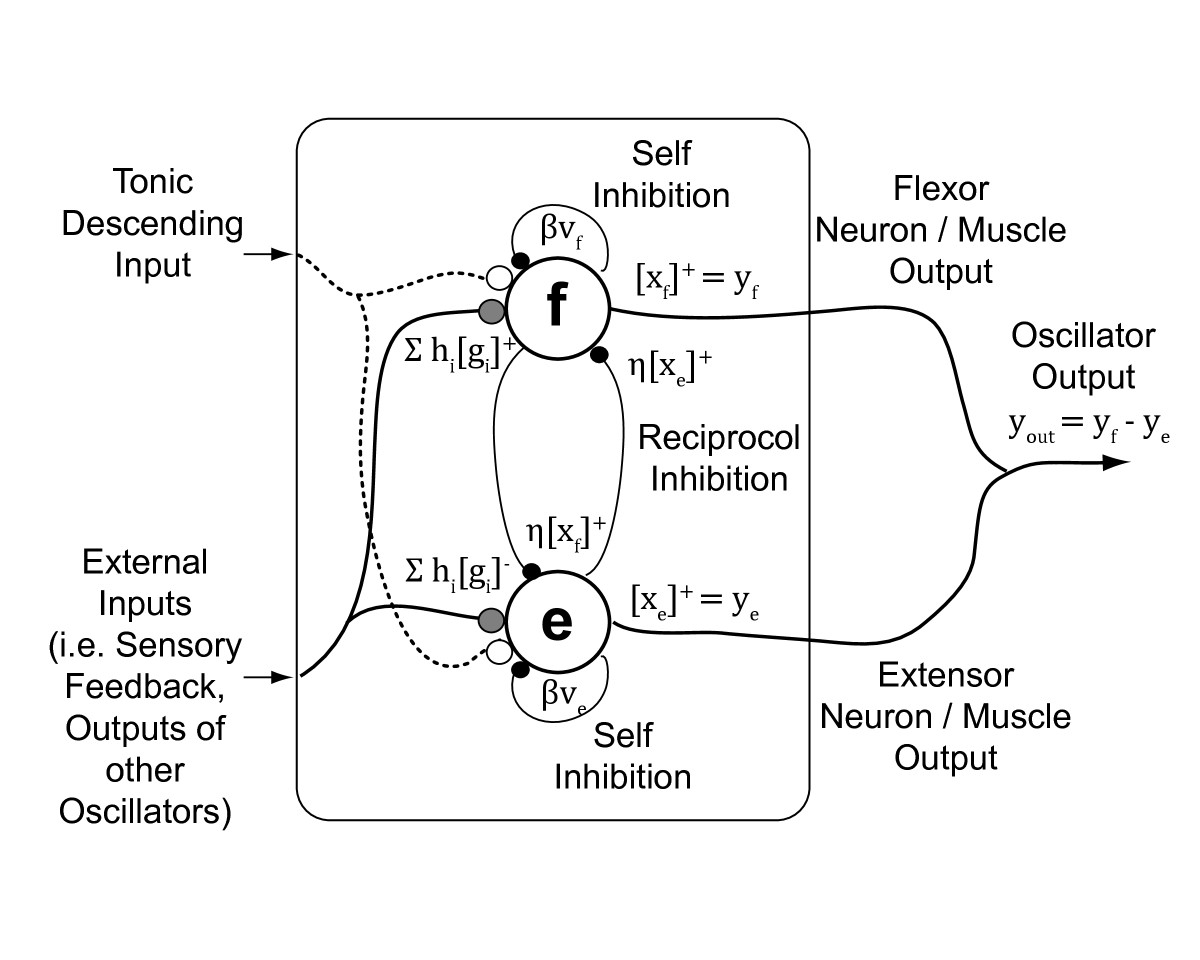
\includegraphics[width=0.7\textwidth]{4}}
					\caption{Matsuoka oscillator \cite{liu2008central}}
					\label{fig:4}
					\vspace{-0.1cm}
				\end{figure}
				
				Two neurons, a flexor (f) and an extensor (e), reciprocally inhibit each other. External inputs ($g_i$) such as sensory feedback or inputs for other neurons can be either inhibitory or excitatory, depending on the gain ($h_i$). Black circles indicate inhibitory inputs. White circles indicate excitatory inputs. Gray circles can be either inhibitory or excitatory.
			\subsubsection{Van der Pol oscillator}
				Van der Pol oscillator benefits are stable limit cycles and relatively interpretable coefficients. Frequency, amplitude and shape coefficients can be identified, although they are not completely independent. Transition between gaits is reached with simple change of oscillator parameters.
				
				The equation of van der Pol oscillator is:
				
				\begin{equation}\label{eq:Pol1}
					\ddot{x} - \epsilon(1 - x^2)\dot{x} + x = 0
				\end{equation}
				
				Where x is the dynamical variable and $\epsilon > 0$ a parameter.
				The van der Pol oscillator has exactly one limit cycle and all other trajectories spiral into it that is proved in \cite{kanamaru2007van}.
			\subsubsection{Rayleigh oscillator}
				Rayleigh oscillator is similar to Van der Pol oscillator but it has reduced sensory requirements, that is an advantage over conventional prosthetic systems.
				
				The equation of Rayleigh oscillator is:
				
				\begin{equation}\label{eq:Rel1}
					\ddot{x} + \epsilon(3x^2 - 1)\dot{x} + (\omega^2 - \epsilon)x = 0
				\end{equation}
			\subsubsection{Spiking Integrate and Fire with Adaption neurons}
				Spiking Integrate and Fire with Adaption neurons were used in \cite{russell2007configuring} for biped locomotion. The CPG was a hierarchical structure of hip timing, knee timing and output patterning. This structure allowed to tune parameters of every of three hierarchical part, and so to configure walking frequency, gait and joint angles independently.
		\section{Neural Networks}
		Despite of the fact that oscillators can be described as a neural network they do not require any input for their work. Canonical Neural Networks (NN) have input data and output. There are several groups of NN.

			\subsection{Feed-Forward Networks}
				In this networks each neuron has its own connection and transfer function. They a ready for state motion generation.  Input data is current kinematics and sensory data. They can generate not state based trajectories only with time input. 
				\subsubsection{Multi-layer perceptron}
					Multi-layer perceptron (MLP) is one of such models. They have from three (input, output, hidden) layers and can have more hidden ones. According to \cite{vundavilli2010dynamically}, two MLPs were used to specify parameters of a bipedal ditch crossing gait trained with Genetic Algorithm (GA). It produced the best solution in terms of stability. It was more stable and efficient than one from a fully analytical approach, and slightly better than the result obtained with a fuzzy logic based method. Activation function of perceptron is sigmoid function.
				\subsubsection{Radial Basis Function Network}
					Radial Basis Function Network is another example of Feed-Forward Networks (FFN). Activation function is usually Gaussian or Euclidean. Neurons in hidden layers connected only with small part of input neurons. For this reason two types of vectors are necessary: wights vector and centre vector which is the same dimension as input. Each vector responds if it is close to its weight vector. Output neurones are the functions of linear combinations of outputs of network and their wighted connections.
					It was used for hexapod locomotion \cite{ilg1995learning}.
				\subsubsection{Cerebellar Model Articulation Controller}
					A Cerebellar Model Articulation Controller (CMAC) is a type of associative memory network based on cerebellum \cite{albus1975new}. Input space is continuous and divided into hyper-rectangles. So input should be located at one rectangle in the moment. Numerous hidden layers are slightly moved rectangles. Hence rectangles will overlap on different layers. The output for each layer is wighted sum of activated rectangles. The CMACs successfully learned the movement patterns and showed resilience to perturbation (including on uneven or slippery floors), thereby translating a rigid analytical solution into an adaptable one \cite{sabourin2005robustness}.
			\subsection{Recurrent Networks}
				The structure of such networks is more complicated that FFN. Thus we can produce more complex patterns and handle different type input.
				
				For recurrent networks there are different types of input and the difference between FFN is that pattern is not required to be provided as an input but it is generated , tuned or chosen internally by the inputs. 
				
				\subsubsection{Jordan and Elman Recurrent NN}
					Jordan recurrent NN is similar to FFN, the difference is that output of the network is recurrently fed to the input.\\
					Elman recurrent NN the difference from Jordan recurrent NN is that delayed output of hidden layer is connected with input of hidden layer. The Elman network was used in \cite{berns1995neural}, the resilient back-propagation training algorithm was used and the system showed an ability to learn supervised trajectories and interpolate between them. The example of Elman recurrent NN is shown on \ref{fig:5} 
					
					\begin{figure}[h!]
						\vspace{-0.2cm}
						\centering
						\begin{tikzpicture}[-,>=stealth',shorten >=1pt,auto,node distance=3cm,
							thick,main node/.style={circle,draw,font=\sffamily\Large\bfseries}]
							
							\node (1) {};
							\node[main node] (2) [right of=1] {$x_1$};
							\node[main node] (3) [right of=2] {$y_1$};
							\node[main node] (4) [right of=3] {$z_1$};
							\node (5) [right of=4] {$b_1$};
							\node (6) [below of=1] {};
							\node[main node] (7) [below of=2] {$x_2$};
							\node[main node] (8) [right of=7] {$y_2$};
							\node[main node] (9) [right of=8] {$z_2$};
							\node (10) [right of=9] {$b_2$};
							\node (11) [below of=6] {};
							\node[main node] (12) [below of=7] {$x_n$};
							\node[main node] (13) [right of=12] {$y_n$};
							\node[main node] (14) [right of=13] {$z_n$};
							\node (15) [right of=14] {$b_n$};
							\node[main node] (16) [below of=13] {$u_1$};
							\node[main node] (17) [below of=16] {$u_2$};
							\node[main node] (18) [below of=17] {$u_3$};
							
							\path[every node/.style={font=\sffamily\small}]
						    	(1) edge node {$in_1$} (2)
								(2) edge node {$w_{x_1y_1}$} (3)
							         edge node {} (8)
							         edge node {} (13)
							    (3) edge node {$w_{x_1z_1}$} (4)
									 edge node {} (9)
									 edge node {} (14)
							    (6) edge node {$in_2$} (7)
							    (7) edge node {} (3)
									 edge node {} (8)
									 edge node {} (13)
								(8) edge node {} (4)
								     edge node {} (9)
								     edge node {} (14)
								(11) edge node {$in_n$} (12)
								(12) edge node {} (13)
								       edge node {} (8)
								       edge node {} (3)
								(13) edge node {} (14)
								       edge node {} (9)
								       edge node {} (4);
							\path[->, every node/.style={font=\sffamily\small}]
						  	    (3) edge [bend left] node[right] {} (16)
						  	    (8) edge [bend left] node[right] {} (17)
						  	    (13) edge [bend left] node[right] {} (18)
								(4) edge node {} (5)
								(9)	edge node {} (10)
                                (14) edge node {} (15)
                                (16) edge [bend left] node[right] {} (3)
                                (17) edge [bend left] node[right] {} (8)
                                (18) edge [bend left] node[right] {} (13);
                             \path[draw=white]
	                             (7) edge node {$\vdots$} (12)
	                             (8) edge node {$\vdots$} (13)
	                             (9) edge node {$\vdots$} (14)
	                             (17) edge node {$\vdots$} (18);
						\end{tikzpicture}
						\caption{Elman recurrent NN}
						\label{fig:5}
						\vspace{-0.1cm}
					\end{figure}
					
				\subsubsection{Fully Connected Recurrent NN}
					In several works \cite{reil2002evolution}, \cite{petridis1994recurrent} a network of several fully connected leaky-integrator neurons were used as a pattern generator. 
					
					The network was able to learn multiple sinusoidal patterns, selectable by an input level, but evolution took more generations as the number of patterns required increased. Learned patterns were resilient to noise at the inputs, and even if the input was disrupted by a large amount, the output would quickly return to normal when the input was corrected. It was found that a six neuron model was sufficient to store eight different sinusoidal patterns, as long as the form of those patterns was different \cite{wright2014intelligent}.
					
					The problem of GA parameters optimization is that for complex systems a huge amount of generations will necessary. 
				\subsubsection{Reservoir}
					Usually recurrent NN should be as small as possible шт order to simplify parameters tuning. Reservoir network follows different principle. It uses big network with potentially much redundancy. The idea is that during training only output layer is trained and reservoir is unchanged. It works with the following assumption: system dynamics is already present when the network is constructed randomly and the only necessary thing is to adjust weights for it. Thus the training process is very simple, e.g. linear regression.
					
					There is practice \cite{wyffels2009design} of generating trajectories with reservoir taken the human capture data.
		\section{Hidden Markov Model}
			Learning by imitation is one of commonly used approach for bipedal locomotion researches. Obviously, direct copying of movements of operator is impossible due to different kinematic and dynamic characteristics. So, from the operator we can take only the pattern and than imitate it on the robot. Observing is estimating the underlying state variables based on the source system through output data. For this task Hidden Markov Models (HMM) can be used \cite{inamura2004embodied}. 
			
			Recognition algorithm is used for identification of movement. If movement was not identified it is added to database as new. Hidden Markov model provides abstraction of the pattern which is used for motion synthesis.
			
			Although typically used for imitation tasks, HMM have also been employed to detect problematic states.
			
			HMM itself is finite state automaton. It is defined by set of states with initial and final states, transition probability matrix where element $a_ij$ is probability of transition from state i to state j.
			
			In feedback system that defines controller error signal is the input. Controller based on its input generates output signal that is called control signal. In order to obtain finite set of decision patterns, it is necessary to divide control space into finite number of subspaces. According to  \cite{yang1994hidden}, the following steps are necessary to define HMM-based controller:
			
			\begin{enumerate}
				\item
					Correspondence  between control signal and controller input (error signal) can be established because according to definition of HMM control signal depends only on finite number of previous input signals.
				\item 
					Define set of patterns. At each time control signal belongs to one of patterns. Also control signal in each moment of time corresponds to one of the set of k previous input signals.
				\item
					It is necessary to label the data. It means that set of input signals is mapped to the set of possible control signals.
				\item
					Train the model by describing control signals by the data.
				\item
					Collect a set of trained models.
			\end{enumerate} 
			
		\section{Rule based approach}
			After the identification of the current state we can find the next one using rule-based method. For bipeds fuzzy-logic systems were used in some researches \cite{park2003fuzzy}.  Fuzzy logic controller helps to deal with a bit of uncertainty in the environment. And it can be used to vary ZMP position in the support polygon \cite{park2003fuzzy}. For proper work it requires optimization of rules, that was basically chosen \cite{vundavilli2010dynamically}.
			The main idea is to divide the set of all possible combinations of system parameters into the area and for each region of this area define the control function that can be used when system is identified to be in the correspondent state.
		
		
	\chapter{Theory}
		According to literature review there are a lot different approaches for bipedal robot locomotion. In this work several of them would be combined.
		We can define two support phases of walking: single support phase (during this phase only one foot is on the ground) and single support phase (two feet are on the ground simultaneously).
		We can break bipedal locomotion in following phases:
		
		\begin{enumerate}
			\item Initial contact
			\item Loading Response
			\item Mid-stance
			\item Terminal Stance
			\item Pre swing
			\item Initial swing
			\item Mid swing
			\item Late swing			
		\end{enumerate}
		
		One of the most simple models of human during single support phase is cart-table model. That is represented on \cref{fig:6}
		
		\begin{figure}[h!]
			\vspace{-0.2cm}
			\centering
			{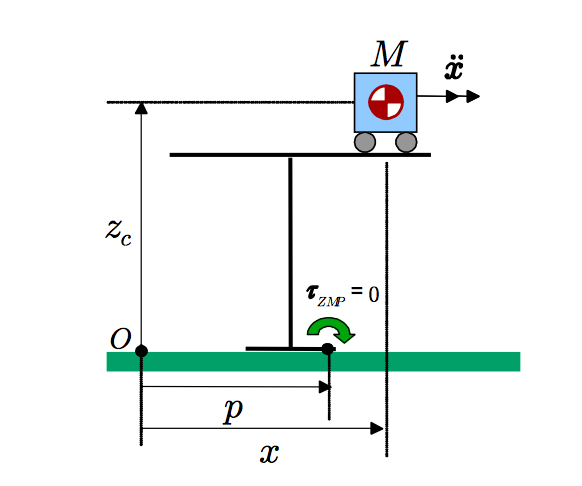
\includegraphics[width=0.7\textwidth]{6}}
			\caption{Cart-table model \cite{kajita2003biped}}
			\label{fig:6}
			\vspace{-0.1cm}
		\end{figure}
		
		When cart is far away from Center of Mass (CoM) that is denoted as X, ZMP point that is denoted as P goes out of support area. When it is happen the system becomes unstable.
		The equation that describes this process was derived in \cite{kajita2003biped} and is represented bellow:
		
		\begin{equation}
			P = X -\dfrac{Z_h}{g} \ddot{X}
		\end{equation}
		
		$Z_h$ here is the height of CoM of the cart.\\
		In order to prevent system failing we want ot control cart in the way that maintains the trajectory of ZMP of the system inside the support polygon. We want this because as were stated in literature survey when ZMP lies in support polygon it maintains the dynamical stability of the system but when it leaves the region of support polygon we have a risk that system will fall. So we can try to define the desired ZMP trajectory of the system. For the beginning we will consider movement only in frontal plane. Frontal plane is represented on \cref{fig:7}. Desired trajectory for our system in frontal plane is provided on \ref{fig:8}.
		
		\begin{figure}[h!]
			\vspace{-0.2cm}
			\centering
			{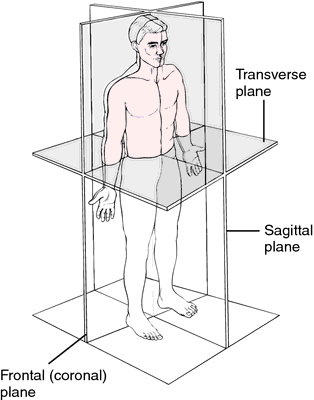
\includegraphics[width=0.7\textwidth]{7}}
			\caption{Human planes [The American Heritage® Medical Dictionary]}
			\label{fig:7}
			\vspace{-0.1cm}
		\end{figure}
		\begin{figure}[h!]
			\vspace{-0.2cm}
			\centering
			{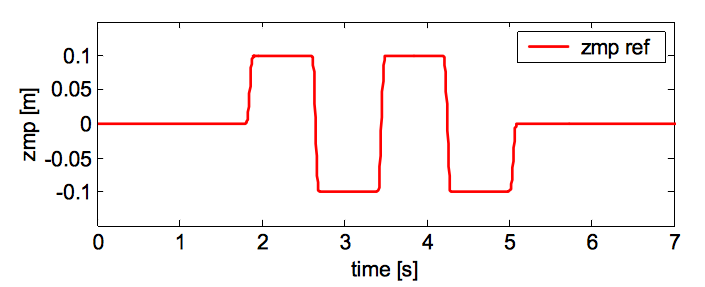
\includegraphics[width=0.8\textwidth]{8}}
			\caption{Desired ZMP trajectory шт frontal plane \cite{kajita2003biped}}
			\label{fig:8}
			\vspace{-0.1cm}
		\end{figure}
		It represents the movement of ZMP from the region of standing foot to the region of swinging foot in the moment of the end of the step. Here the amplitude if frictions is defined by parameters of robot (step width in frontal plane). Thus we can build simple system represented on \cref{fig:9}.
		\begin{figure}[h!]
			\vspace{-0.2cm}
			\centering
			{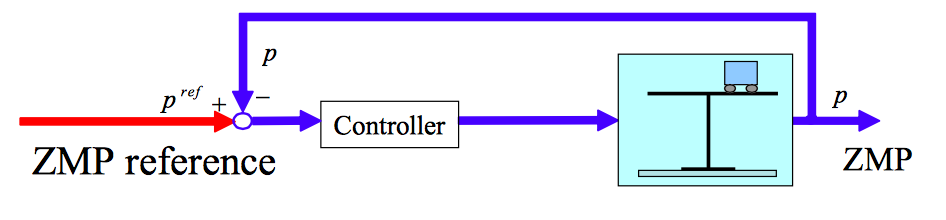
\includegraphics[width=0.7\textwidth]{9}}
			\caption{PID regulated ZMP control \cite{kajita2003biped}}
			\label{fig:9}
			\vspace{-0.1cm}
		\end{figure}
		Where controller is PID (proportional integral derivative) regulator maintains ZMP trajectory to be closed to desired one. We can see that our real ZMP trajectory is late and so CoM trajectory is late too. The result of such control is represented on \cref{fig:10}.
		\begin{figure}[h!]
			\vspace{-0.2cm}
			\centering
			{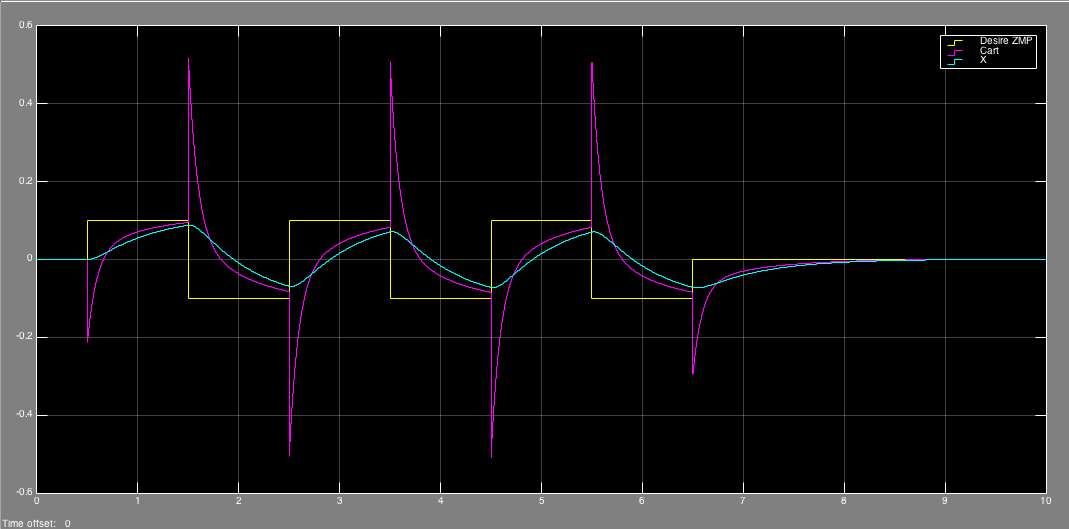
\includegraphics[width=1\textwidth]{10}}
			\caption{PID regulated ZMP trajectories}
			\label{fig:10}
			\vspace{-0.1cm}
		\end{figure}
		Kajita et all in \cite{kajita2003biped} introduced simple idea. To look forward to desired ZMP. And try to predict what will happen before it happens. Hence the theory of optimal control matters and it will be described bellow how to make predictive control system for such unstable object as cart of the table model for example. Further in Chapter 4 such controller would be applied to the model of robot and in Chapter 5 the results will be evaluated.
		
		\section{Optimal control}
			According to \cite{hazell2008discrete} it is necessary to introduce discrete-time state-space model if form \ref{eq:oc1}.
			
			\begin{equation}\label{eq:oc1}
				\begin{split}
					x(k+1) = Ax(k) + Bu(k)\\
					y(k) = Cx(k) + Du(k)
				\end{split}
			\end{equation}
			
			Where k is time index, x(k) is a vector of state values, u(k) is a vector of input values, y(k) is a vector of output values. A,B,C,D are  appropriately dimensioned real matrices \cite{hazell2008discrete}.
			
			We define G - transfer function associated with model \ref{eq:oc1}. G is defined as \ref{eq:oc2}
			
			\begin{equation}\label{eq:oc2}
				G(Z) = C(ZI - A)^{-1}B+D
			\end{equation}
			
			Where Z is Z-transform variable.
			
			We can estimate the size of transfer function by measures that a known as $H_2$ and $H_\infty$. $H_2$ norm will be denoted as $||G(Z)||_2$ and is defined as \ref{eq:oc3}.
			
			\begin{equation}\label{eq:oc3}
				||G(Z)||_2 = Tr\{ B^{'} XB + D^{'} D \}
			\end{equation}
			
			Where X is defined by \ref{eq:oc4}.
			
			\begin{equation}\label{eq:oc4}
				X = A^{'} XA + C^{'} C
			\end{equation}
			
			According to \cite{hazell2008discrete} 	$H_2$ norm of transfer function is a gain in power from input to output, assuming that the input signal is white and Gaussian.  
			
			$H_\infty$ is denoted as $||G(Z)||_\infty$ and is defined by \ref{eq:oc5}.		
			
			\begin{equation}\label{eq:oc5}
				||G(Z)||_\infty = \sup_{\omega} \dfrac{||z||_2}{||\omega||_2}
			\end{equation}
			
			Here $z = G\omega$, $\omega$ is assumed to be a realization of unit power, Gaussian, white-noise process and z is real values vector of input. Hence $H_\infty$ defines maximum possible gain in power from input ot output.
			
			\begin{figure}[h!]
				\vspace{-0.2cm}
				\centering
				{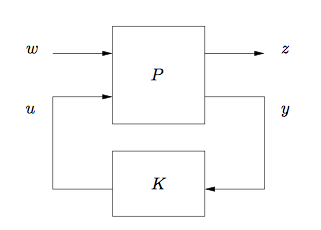
\includegraphics[width=0.7\textwidth]{11}}
				\caption{Generalized regulator \cite{hazell2008discrete}}
				\label{fig:11}
				\vspace{-0.1cm}
			\end{figure}
			
			On \cref{fig:11} there is a generalized regulator. The input for the system is $\omega$. The system is controlled by input signal u and returns output signal z, while y is measurements output.
			
			The matrix equation \ref{eq:oc6}
			
			\begin{equation}\label{eq:oc6}
				X = A^{'}XA + Q - \bar{L}^{'} \bar{R}^{-1} \bar{L}
			\end{equation}
			
			is known as Discrete Algebraic Riccati Equation (DARE). Where $\bar{R} = R + B^{'}XB$. With $\bar{R} = R + B^{'}XB$ and $\bar{L} = L + B^{'}XA$. The solution of this equation are considered and derived in \cite{hazell2008discrete}. Also we can write DARE in a short form: $X = D(A,B,Q,R,L;X)$ and $D(A,B,Q,R,L;X) = A^{'} XA + Q -  \bar{L}^{'} \bar{R}^{-1} \bar{L}$.
		
		\subsection{Preview control} 
			Katayama et al. in \cite{katayama1985design} introduced new method of control general regulators with preview control. The key idea was to look forward for N discrete steps and predict desirable value of controlled signal. The form of control signal was derived by \cite{katayama1985design} and it is given in \ref{eq:pc1}
			
			\begin{equation}\label{eq:pc1}
				u(k) = -G_I \sum^{k}_{i=0} e(i) - G_xx(k) - \sum^{N_l}_{l=1}G_d(l)y_d(k+l)
			\end{equation}
		
			Here $G_I = [R+\tilde{B}^T \tilde{K} \tilde{B}]^{-1} \tilde{B}^T \tilde{K} \tilde{I}$, \\$G_x = [R+\tilde{B}^T \tilde{K} \tilde{B}]^{-1} \tilde{B}^T \tilde{K} \tilde{F}$,\\
			$G_d(1) = -G_I$ and $G_d(l) = [R+\tilde{B}^T \tilde{K} \tilde{B}]^{-1} \tilde{B}^T \tilde{X}(l-1)$.\\
			Moreover $\tilde{K}$ here is a solution of DARE in the form of \ref{eq:pc2}
			\begin{equation}\label{eq:pc2}
				\tilde{K} = \tilde{A}^T\tilde{K}\tilde{A} - \tilde{A}^T \tilde{K} \tilde{B} [R + \tilde{B}^T \tilde{K} \tilde{B}]^{-1} \tilde{B}^T\tilde{K}\tilde{A} + \tilde{Q}
			\end{equation}
			\begin{equation}\label{eq:pc3}
				\begin{split}
					\tilde{B} = \begin{bmatrix} C B \\ B \end{bmatrix}\\
					\tilde{I} = \begin{bmatrix} I_p \\ 0 \end{bmatrix}\\
					\tilde{F} = \begin{bmatrix} CA \\ A \end{bmatrix}\\
					\tilde{Q} = \begin{bmatrix} Q_e & 0 \\ 0 & Q_x \end{bmatrix}\\
					\tilde{A} = \begin{bmatrix} \tilde{I} & \tilde{F} \end{bmatrix}
				\end{split}
			\end{equation}
			
			And finally $I_p$ is $p * p$ identity matrix.
			
			This theorem was proven in \cite{katayama1985design}. And Kajita et al. in \cite{kajita2003biped} proved, that the necessary prediction for the system is 1.6 seconds due to the character за dependency on this parameter that is shown on \cref{fig:12} 
			
			\begin{figure}[h!]
				\vspace{-0.2cm}
				\centering
				{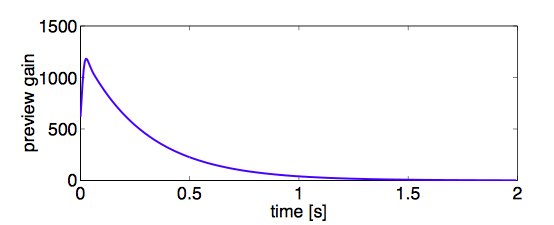
\includegraphics[width=0.7\textwidth]{12}}
				\caption{Importance of N preview \cite{kajita2003biped}}
				\label{fig:12}
				\vspace{-0.1cm}
			\end{figure}
	\chapter{Implementation}
		Initially the model of cat-table was developed. The design is represented on \cref{fig:13}
		\begin{figure}[h!]
			\vspace{-0.2cm}
			\centering
			{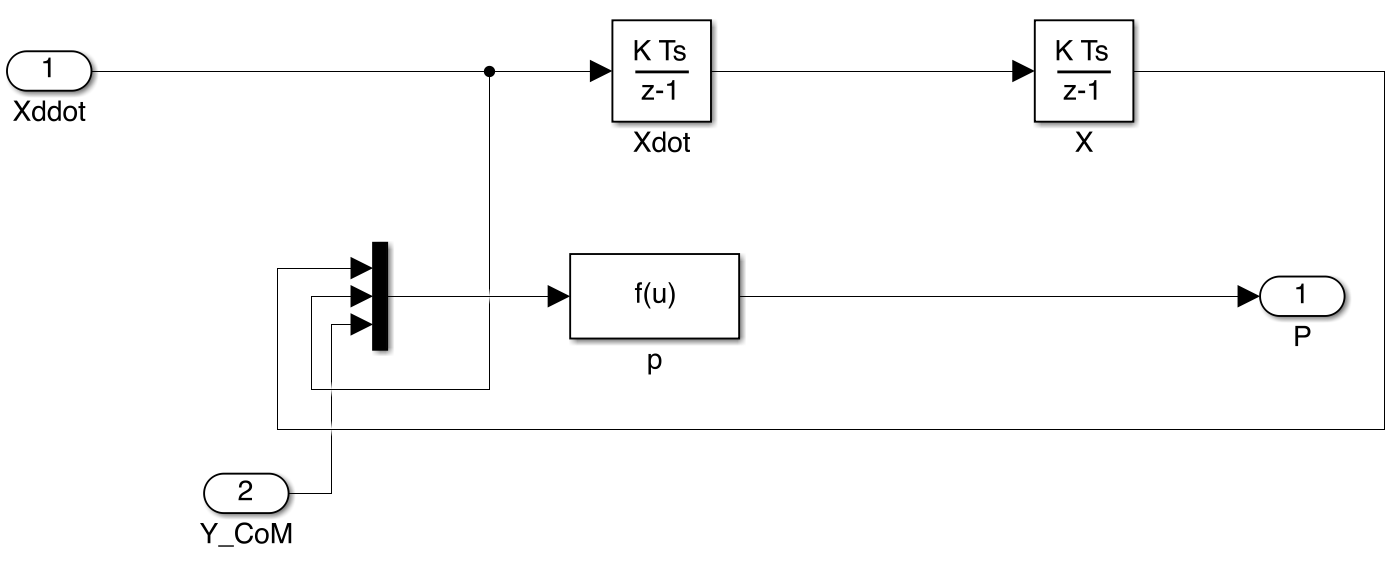
\includegraphics[width=0.7\textwidth]{13}}
			\caption{Cart-table model}
			\label{fig:13}
			\vspace{-0.1cm}
		\end{figure}
		
		Further it will be represented as block on \cref{fig:14}.
		
		\begin{figure}[h!]
			\vspace{-0.2cm}
			\centering
			{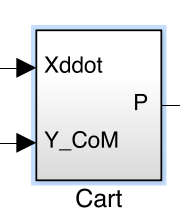
\includegraphics[width=0.3\textwidth]{14}}
			\caption{Cart-table model block}
			\label{fig:14}
			\vspace{-0.1cm}
		\end{figure}
		
		To have the initial control model Propotional Integral Derivative (PID) regulator was applied. The system of PID regulated cart-table model is on \cref{fig:15}.
		
		\begin{figure}[h!]
			\vspace{-0.2cm}
			\centering
			{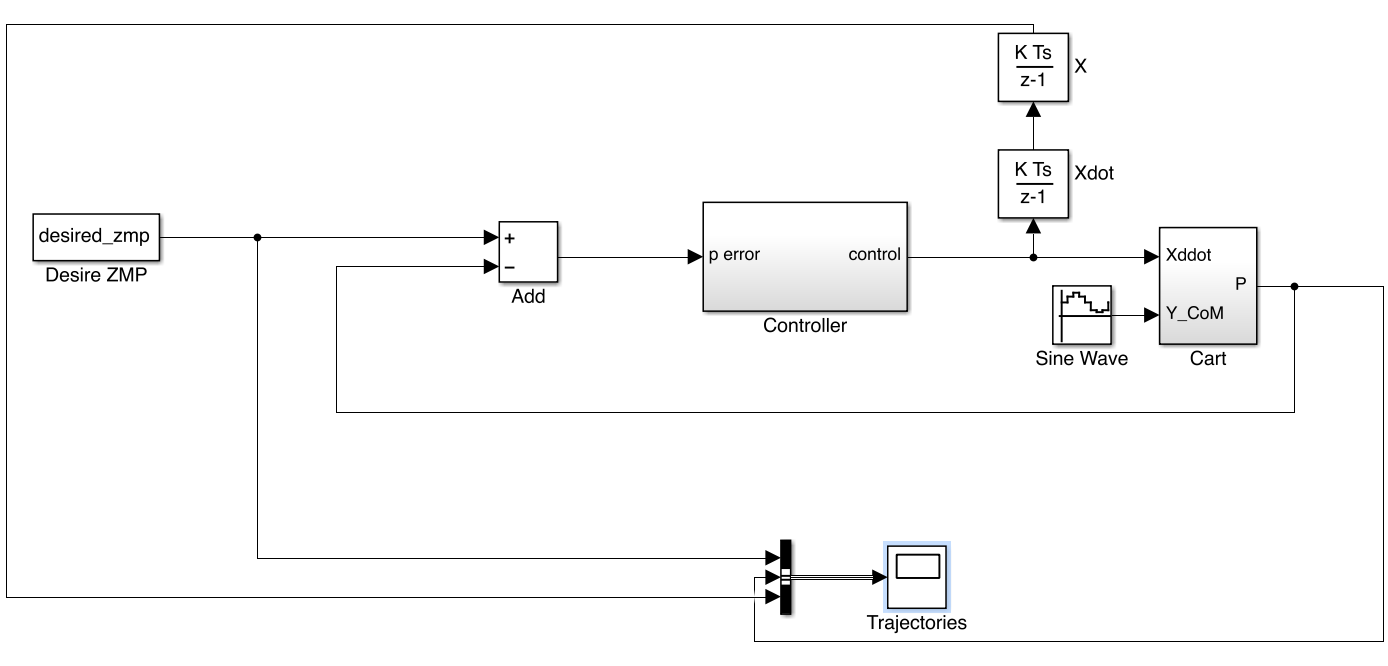
\includegraphics[width=1\textwidth]{15}}
			\caption{PID regulated cart-table}
			\label{fig:15}
			\vspace{-0.1cm}
		\end{figure}
		
		And the regulator itself looks as on \cref{fig:16}.
		
		\begin{figure}[h!]
			\vspace{-0.2cm}
			\centering
			{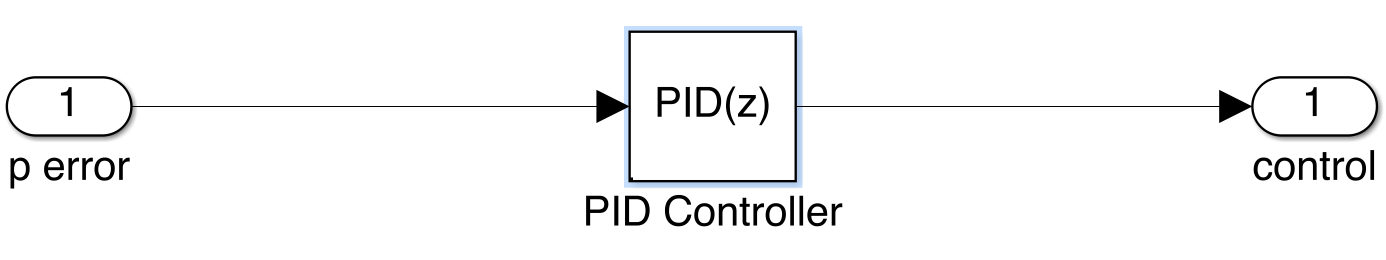
\includegraphics[width=0.7\textwidth]{16}}
			\caption{PID regulator of cart-table}
			\label{fig:16}
			\vspace{-0.1cm}
		\end{figure}
		
		The results of such control are represented on \cref{fig:17}.
		
		\begin{figure}[h!]
			\vspace{-0.2cm}
			\centering
			{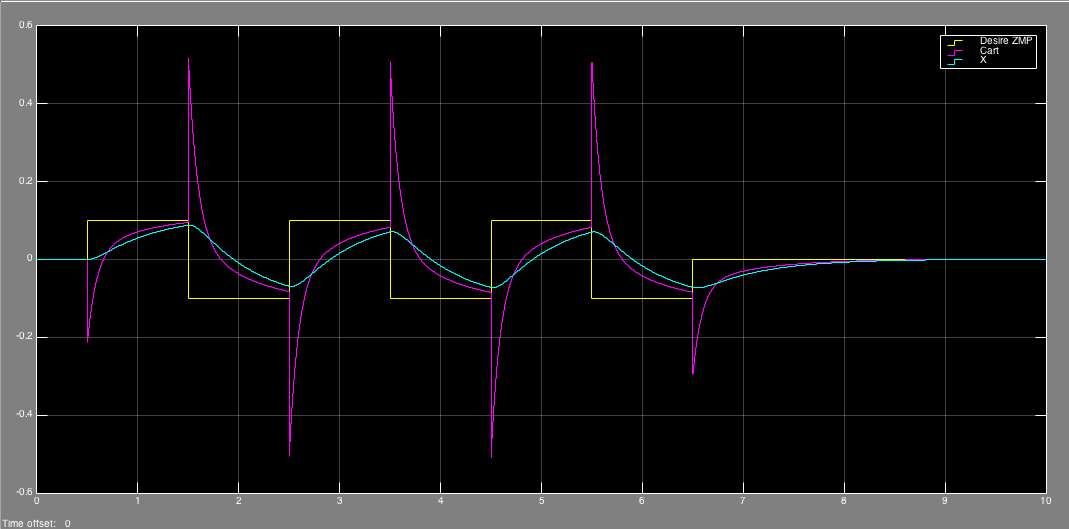
\includegraphics[width=0.8\textwidth]{17}}
			\caption{PID regulator control results}
			\label{fig:17}
			\vspace{-0.1cm}
		\end{figure}
		
		We can see that actual ZMP trajectory lates and due to this fact the CoM trajectory reaches the bound of support polygon and thus it makes the system unstable.
		
		After that preview control with 1.6s prediction was applied. The difference between PID controlled model is only in the controller, that is represented on \cref{fig:18}.
		
		\begin{figure}[h!]
			\vspace{-0.2cm}
			\centering
			{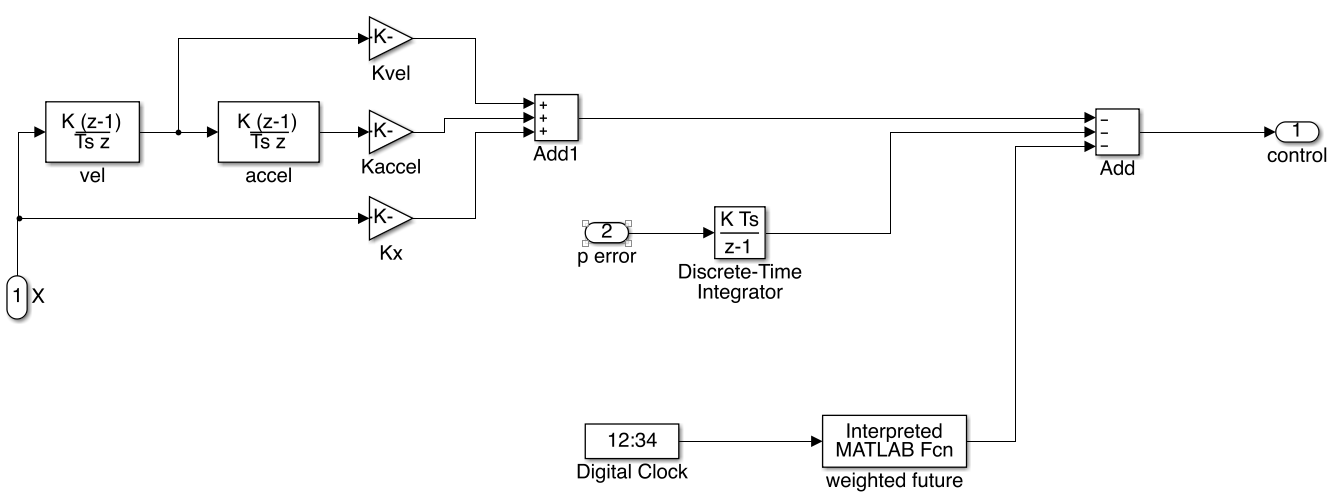
\includegraphics[width=1\textwidth]{18}}
			\caption{Preview controller design}
			\label{fig:18}
			\vspace{-0.1cm}
		\end{figure}
		
		The results of this controller are represented on \cref{fig:19} are much better and we can see only no late response and no overshooting in ZMP trajectory. Thus the system become much more stable than in PID case. 
		
		\begin{figure}[h!]
			\vspace{-0.2cm}
			\centering
			{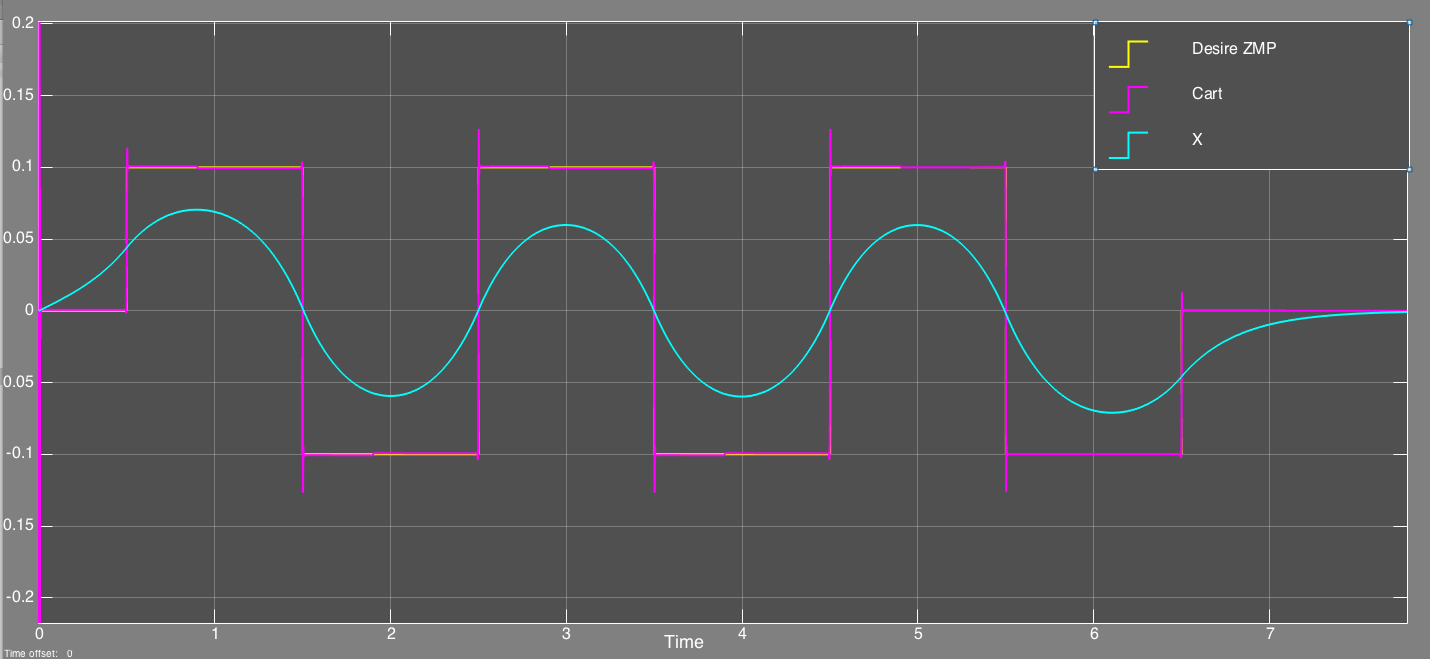
\includegraphics[width=0.7\textwidth]{19}}
			\caption{Preview controller results}
			\label{fig:19}
			\vspace{-0.1cm}
		\end{figure}
	\chapter{Evaluation}
	\chapter{Future work}
	\chapter{Summary}
	
	\bibliographystyle{unsrt}
	\bibliography{robotics}
	
	\begin{appendices}
		\chapter{Preview control parameters estimation algorithm}
			\begin{lstlisting}
function [Ke, Kx, G] = preview_control_params(T, Zh, N)
	R = 1e-6;
	Qe = 1;
	Qdpos = 0;
	Qdvel = 0;
	Qdaccel = 0;
	g = 9.8;
	
	A = [1 T T^2/2;0 1  T;0 0 1];
	B = [T^3/6;T^2/2;T];
	C = [1 0 -Zh/g];
	
	AA = vertcat(horzcat([1], C*A),horzcat(zeros(3,1), A));
	BB = vertcat([C*B], [B]);
	RR = R;
	QQ = diag([Qe, Qdpos, Qdvel, Qdaccel]);
	
	PP = dare(AA,BB,QQ,RR);
	SS = 1.0/(RR + BB'*PP*BB);
	KK = SS*BB'*PP*AA;
	
	Ke = KK(1,1);
	Kx = KK(1,2:4);
	
	Ac = AA - BB*KK;
	XX = -Ac' * PP * [1,0,0,0]';
	
	G = [-Ke];
	
	for i=2:1:N
		G = [G SS * BB' * XX];
		XX = Ac' * XX;
	end
end
			\end{lstlisting}
		\chapter{Robot constants and desired ZMP generation algorithm}
			\begin{lstlisting}
g = 9.8;
Zc = 1;
T = 1e-4;
N = 16000;
sim_time = 10;

[Ke, Kx, G] = preview_control_params(T, Zc, N);

D_o = [1 3 5]';                % delays
D_e = [2 4 6]';                % delays
t = 0 : T : sim_time + N * T;  % signal evaluation time
width = 1;                     % width of each pulse

desired_zmp = 0.1 * pulstran(t, D_o, 'rectpuls', width)\
- 0.1 * pulstran(t, D_e, 'rectpuls', width);
desired_zmp = [t' desired_zmp'];
			\end{lstlisting}
	\end{appendices}
  
\end{document}